% =====================================================================
% draft.tex — "A New Class of Cellular Automata"
%
% A RESULTS paper, refactored from main.tex (which is an exploration note).
% Joe, 2026-07-17: "I bet we could write a straightforward five-to-ten-page
% paper, including pictures. Rather than 'What Undecidability Feels Like From
% the Inside' I might call it 'A new class of cellular automata'."
%
% WHAT CHANGED, and why. main.tex is 1,197 lines built around a fail bank —
% Joe: "even the fail bank sounds like exploratory data analysis". This keeps
% only what survives as a RESULT and demotes the negatives to the one paragraph
% that explains them.
%
% IN:   the object; the parity theorem; the closed form; fixed-byte counts = 2^k;
%       the census (5x death, monotone in k); the prospective test (reduced
%       rotate+2); bias-not-absorber; the interrupter; and the headline —
%       EVERY FIXED POINT SITS AT LANGTON'S lambda = 1/2, exactly, all 40,320,
%       zero violations, with a two-line proof.
% OUT:  transfer (never shown); the tokamak (cascade 0/12 = identity 0/12, not a
%       win, per lon-claude-6's own control); the duet (MI null); the policy
%       population (blend fired 0.2% of calls); C_mu (a frozen barcode beats
%       Rule 110); the heads (dose 1/80).
% DEMOTED: the three-metric fail bank -> one paragraph. Parity is not a metric
%       property, so distance-geometry cannot see it. That is an explanation,
%       not twenty pages.
% =====================================================================
\documentclass[man,12pt,floatsintext]{apa7}

\usepackage[american]{babel}
\usepackage{csquotes}
\usepackage{amsmath,amssymb}
\usepackage{amsthm}
\usepackage{booktabs}
\usepackage{graphicx}
\usepackage{xcolor}
\usepackage{subcaption}
\usepackage[style=apa,backend=biber]{biblatex}
\addbibresource{refs.bib}

\newcommand{\sig}{\sigma}
\newcommand{\bit}[1]{\mathrm{bit}[#1]}
\newtheorem{theorem}{Theorem}
\newtheorem{corollary}[theorem]{Corollary}

\title{A New Family of Operators on Cellular Automata}
\shorttitle{A New Family of Operators on Cellular Automata}
\author{Joseph Corneli}
\affiliation{}

\abstract{%
We describe a cellular automaton whose cells do not hold states but
\emph{rules}, and an operator that rewrites those rules by acting on the
rule's own truth table: $\bit{\sig(k)} := \lnot\,\bit{k}$ for $\sig$ a
permutation of the eight neighbourhoods. The rule's truth table is itself
an eight-cell automaton whose topology is $\sig$ --- an automaton inside
the automaton --- giving a family of $8! = 40{,}320$ operators that is
finite, exhaustively enumerable, and exactly classified.

The classification is by cycle parity. A Boolean fixed point of $\sig$
exists if and only if every cycle of $\sig$ is even; the count of such
$\sig$ is $((2n-1)!!)^2$, which for $S_8$ gives $105^2 = 11{,}025$ of
$40{,}320$, or $27.34\%$. A census of all $20{,}256$ mirror orbits
confirms the proportion to two decimal places and shows the all-even class
dying five times as often as the rest.

The main result concerns where those fixed points \emph{are}. Every fixed
point of every operator in the family --- all $40{,}320$ of them, with no
exceptions --- has exactly four one-bits, hence Langton's
$\lambda = 1/2$. This is forced: an alternating colouring assigns each
even cycle of length $2m$ exactly $m$ ones, so the total is $8/2 = 4$
necessarily. Langton's critical value, obtained empirically as a statistic
over rule space and long contested, appears here as an exact consequence
of a fixed-point condition. Operators with all-even cycle structure possess
these attractors; operators with any odd cycle possess none.

Possessing an attractor at $\lambda = 1/2$ is not, however, the same as
sustaining edge-of-chaos behaviour---the all-even class in fact preferentially
\emph{dies}, settling onto its attractors---and because every attractor
shares the one value, $\lambda$ cannot itself distinguish the operators that
hold a complex population from those that collapse. That distinction we carry
with an endogenous, population-level analogue of $\lambda$: the trajectory of
rule diversity in the driven field, which separates sustained from transient
edge-of-chaos across the family.}

\begin{document}
\maketitle

\section{The Object}
\label{sec:object}

A cellular automaton normally evolves a field of \emph{states} under one
fixed rule. Invert that arrangement: let each cell hold a \emph{rule}, and
let an operator evolve the field of rules. An elementary cellular automaton
(ECA) rule is an eight-bit truth table $\bit{k}$, with $k$ ranging over the
eight three-cell neighbourhoods. We study the operator, parameterised by a
permutation $\sig \in S_8$ that acts on the rule's own table:
\begin{equation}
\bit{\sig(k)} := \lnot\,\bit{k}.
\label{eq:prop}
\end{equation}
The truth table is thereby itself an eight-cell automaton whose wiring is
$\sig$ and whose update is Boolean negation --- an automaton inside the
automaton. Equation~\eqref{eq:prop} defines a family of $8! = 40{,}320$
operators that is finite, exhaustively enumerable, and, as we show below,
exactly classified.

The substrate---a cellular automaton whose cells hold rules rather than
states---is not itself new \parencite{corneli2015search}; what we introduce
is the \emph{operator} of Equation~\eqref{eq:prop}, understood as an
enumerated, exactly classified family. That 2015 paper found a single
member of this family, encountered through a programming error and not
recognised as one of many; we now give the family an essentially complete
characterisation. The canonical symmetry group of ECA
rule space has order four (reflection $\times$ complement, collapsing $256$
rules to $88$ classes) \parencite{svozil2025symmetries}; it is not $S_8$,
and the negation-carrying, $\sig$-parameterised family of
Equation~\eqref{eq:prop} does not appear in it. Rule-space permutation as a
parameterised, enumerated family with a derived fixed-point structure does
not appear in the literature we have surveyed; the nearest neighbours
augment cellular automata with state-dependent feedback
\parencite{pavlic2014selfref} rather than permuting the rule itself. Two
established genres are adjacent but distinct: per-cell rules (non-uniform or
$\nu$-CA \parencite{dennunzio2011nonuniform}) and rules that change during
evolution (rule-changing or programmable CA
\parencite{mori1998rulechanging}). A
referee should note the trap in the first: a $\nu$-CA drawing rules from a
finite set is equivalent to a uniform CA on the product alphabet
\parencite{dennunzio2011nonuniform}, so the substrate is not where novelty
lives. It lives in the fixed-point structure of the operator, which is what
the rest of this paper is about.

\begin{figure}[tp]
\centering
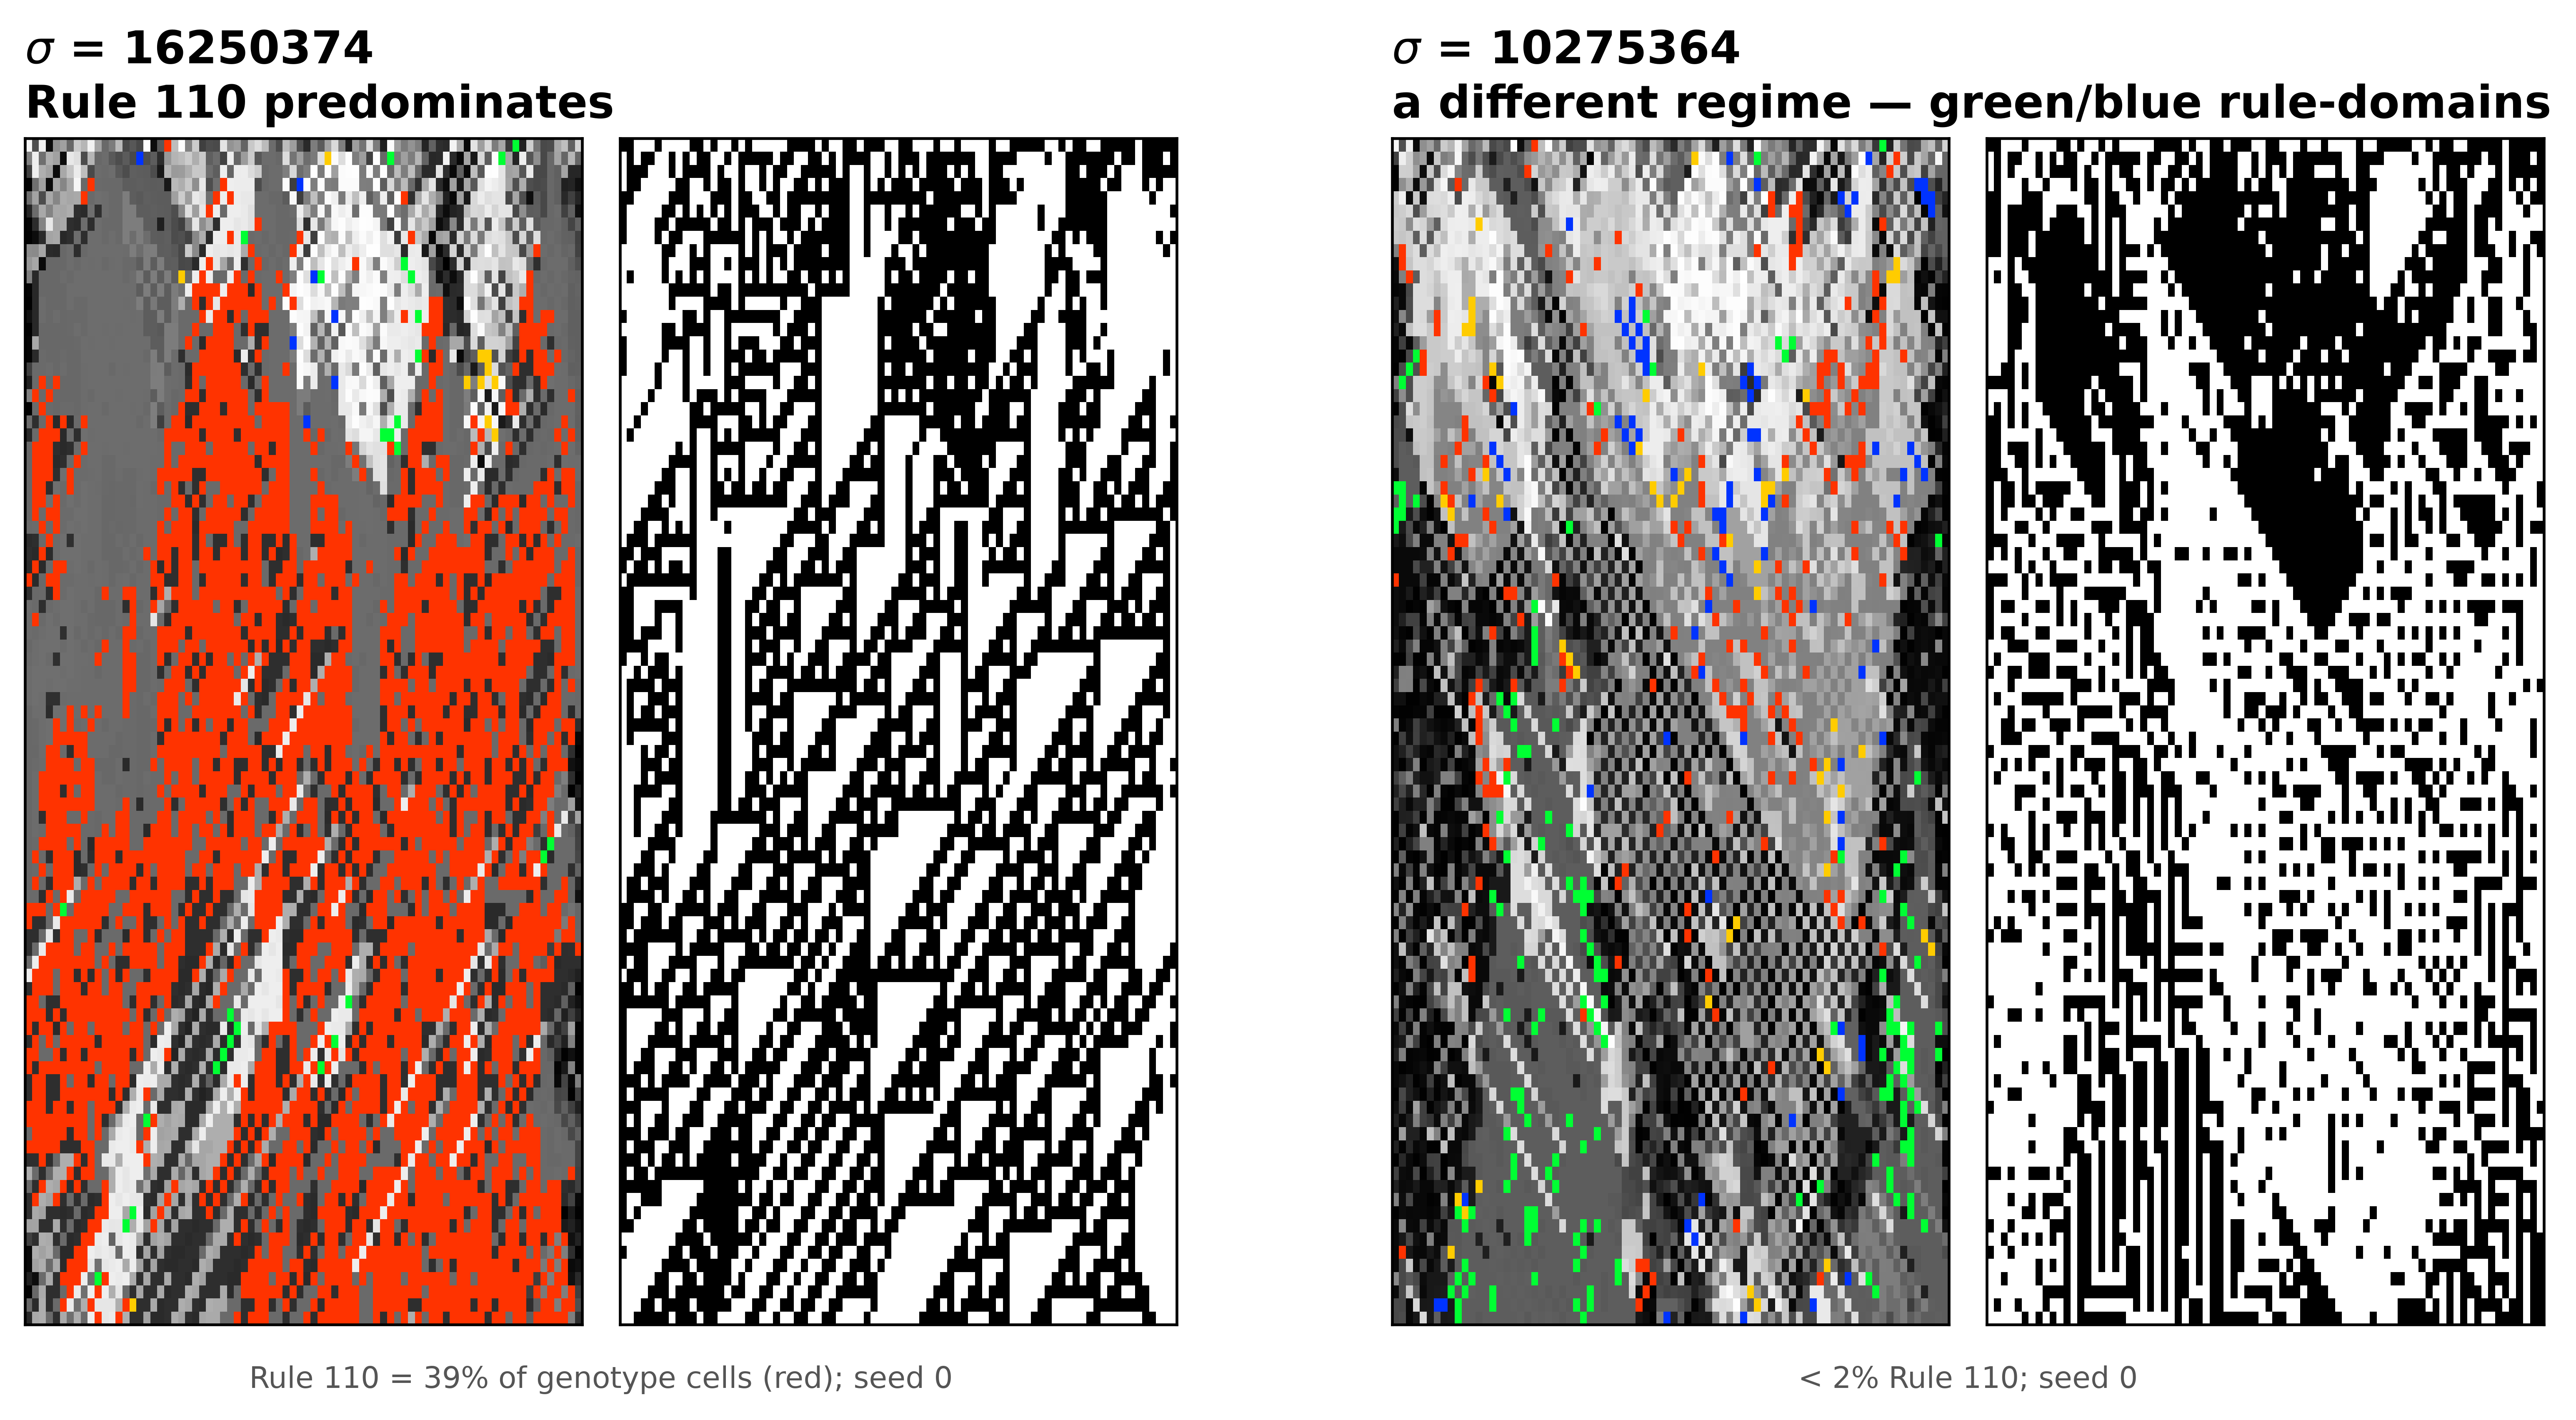
\includegraphics[width=\linewidth]{figures/rule110_spread.png}
\caption{Two operators from the family, each shown over time as genotype
(256-colour, left) and phenotype (black and white, right). Under
$\sig = 16250374$ the genotype field comes to be dominated by ECA
Rule~110---the red cells, $34\%$ of the genotype---and the phenotype
accordingly displays Rule~110's characteristic gliders; under
$\sig = 10275364$ a different regime of rule-domains forms (green and blue,
under $2\%$ Rule~110). The operator does not merely stir rule space: it
drives it toward particular, computationally distinguished rules. Genotype
colours are the legacy engine's own.}
\label{fig:regimes}
\end{figure}

\section{The Classification}
\label{sec:classification}

\subsection{Fixed points exist iff every cycle is even}

\begin{theorem}\label{thm:parity}
The operator~\eqref{eq:prop} has a Boolean fixed point if and only if $\sig$
is fixed-point-free and every cycle of $\sig$ has even length.
\end{theorem}

\noindent A fixed point is a rule invariant under~\eqref{eq:prop}, i.e.\ a
$\sig$-equivariant Boolean colouring $g$ with $g(\sig k) = \lnot\,g(k)$.
Follow a cycle of length $L$: equivariance forces
$g(k) = (\lnot)^{L} g(k)$, and $(\lnot)^{L}$ is the identity exactly when
$L$ is even; conversely, colour each orbit by the parity of its distance
from a chosen representative. A fixed point ($L=1$) is odd and so admits no
such colouring, which is why the fixed-point-free condition is required.

This is the signed-cycle fixed-point theorem of Boolean-network theory
\parencite{aracena2008maximum} specialised to~\eqref{eq:prop}: our operator
is a Boolean network whose signed interaction digraph is $\sig$ with every
arc negative, a negation-cycle of length $\ell$ has sign $(-1)^\ell$, and
an isolated negative cycle admits no fixed point while a positive (even)
one admits exactly two. We contribute a machine-checked proof of the
specialised statement in Lean~4 / Mathlib.\footnote{%
\texttt{DarkTower/Patterns/Propagator.lean}, theorem
\texttt{hasAlternatingColouring\_iff\_cycleType\_even}; \texttt{lake build}
clean, no \texttt{sorry} or \texttt{axiom}.}

\subsection{The closed form}

The number of $\sig \in S_{2n}$ with all cycles even is $((2n-1)!!)^2$,
generated by $1/\sqrt{1-x^2}$ (the ``set of even cycles'' construction).
For $S_8$ this is $105^2 = 11{,}025$ of $40{,}320$, or $27.34\%$. The count
is classical: it is \textcite{oeis_a001818} and appears as
\textcite[Problem~5.34(c)]{stanley1999enumerative} and in
\textcite{riordan1968combinatorial}. We claim it only as the enumeration of
our operator family, not as a new identity.

\subsection{Fixed bytes number $2^k$}

An all-even $\sig$ with $k$ cycles has exactly $2^k$ fixed bytes; any
$\sig$ with an odd cycle has none. Each even cycle admits exactly two
alternating colourings, chosen independently across cycles, whence $2^k$;
the zero case is Theorem~\ref{thm:parity}. This too is machine-checked.%
\footnote{\texttt{alternatingColouring\_card\_eq\_two\_pow\_cycleType\_card}.}
Summed against these weights the family is consistent:
$\sum 2^{k}$ over all-even $\sig$ equals $(2n)! = 8! = 40{,}320$, the total
number of fixed bytes across the family.

\section{Langton's $\lambda$ Is a Fixed-Point Condition}
\label{sec:lambda}

Langton's $\lambda$ measures a rule's \emph{activity}: the fraction of its
neighbourhood entries that map to the non-quiescent
state~\parencite{langton1990computation}. For an eight-bit ECA table it is
the Hamming weight over eight, $\lambda = \lVert r \rVert_1 / 8$, running
from $0$ (every neighbourhood dies) through $1/2$ to $1$. Langton's thesis
was that complex, computation-supporting behaviour concentrates near a
critical value; for the two-symbol case that value is $1/2$.

\subsection{Every fixed point has $\lambda = 1/2$}

\begin{theorem}\label{thm:lambda}
Every fixed point of every operator in the family has exactly four one-bits;
equivalently, Langton's activity parameter $\lambda = 4/8 = 1/2$.
\end{theorem}

\noindent By Theorem~\ref{thm:parity} each cycle has even length $2m$; an
alternating colouring assigns such a cycle exactly $m$ ones; summing over
cycles gives $(\sum L)/2 = 8/2 = 4$. Exhaustive enumeration confirms it:
across all $40{,}320$ operators and all their fixed points, every one has
Hamming weight four, with zero exceptions. The statement is machine-checked
for $\mathrm{Fin}\,8$.\footnote{%
\texttt{alternatingColouring\_true\_card\_eq\_four}: the true-cells and
false-cells are put in bijection by $\sig$, forcing each to number four.}

We are deliberate about the standing of this result. Langton's critical
value was obtained empirically, as a statistic over rule space
\parencite{langton1990computation}, and its status as an order parameter
was contested: \textcite{mitchell1993revisiting} refuted
\textcite{packard1988adaptation}'s specific genetic-algorithm clustering
claim, not the definition of $\lambda$, which survived as one axis among
others such as Wuensche's $Z$ \parencite{wuensche1999classifying} and
Voorhees's $\Theta$. There is a folklore intuition for why $1/2$
is special --- binomial sampling variance $\lambda(1-\lambda)$ is maximal
there --- and it is not ours; and it has been noted that $\lambda$ alone
does not fix a rule's dynamical class, distinct classes coexisting at a
single value \parencite{sakai2002edge}. What
Theorem~\ref{thm:lambda} adds is that under the complementation
in~\eqref{eq:prop} the value $1/2$ is \emph{forced}: any
alternation-under-complement construction lands there by parity. We present
it not as a surprising discovery but as an exact and elementary consequence
of the operator's fixed-point condition --- which is precisely what makes
it a theorem rather than a measurement.

\subsection{The cast: which rules survive, and how many}

Under an all-even $\sig$, the rules that \emph{survive}---that the operator
maps to themselves, and onto which the driven field settles in the long
run---are exactly its fixed points. Their number is $2^k$, where $k$ is the
number of cycles of $\sig$ (\S\ref{sec:classification}): each even cycle
admits two alternating colourings, and they are chosen independently across
cycles. Every survivor has $\lambda = 1/2$ (Theorem~\ref{thm:lambda}), so
the surviving population is a cast of \emph{distinct} rules---distinct truth
tables---sharing a \emph{single} activity.

The smallest nontrivial case of the count is a single cycle, $k = 1$: two
survivors. The 2015 paper's Figure~8 already exhibited a two-rule residual
(Figure~\ref{fig:figure8}): a random field of tens of distinct rules dies
off to an alternating population of just two, rules $42$ and $170$.
Fittingly, the programming error that produced the family is what pins its
residual at two---the erroneous mutation froze a bit, splitting the field
into the cells that can reach $42$ and those that can reach $170$---so the
phenomenon was on the page before the $2^k$ count explained it.

That die-off curve---the count of distinct rules over time---is the natural
population-level analogue of $\lambda$. Where $\lambda$ is a scalar assigned
to a single rule and swept across an ensemble to locate the edge of chaos,
this curve is an \emph{endogenous} order parameter: the driven field's own
path through rule space. And where $\lambda$ is exhausted here---every
survivor sits at $1/2$---the curve still discriminates, because it measures
the population rather than the point. Read across a whole family it
separates sustained from transient edge-of-chaos
(\S\ref{sec:interrupter}, Figure~\ref{fig:lambda}).

Diversity of the surviving population and singularity of its activity
coexist, and no distance detects the first (\S\ref{sec:metrics}). Diversity of the surviving population and singularity of its
activity coexist, and no distance detects the first (\S\ref{sec:metrics}).

\begin{figure}[t]
\centering
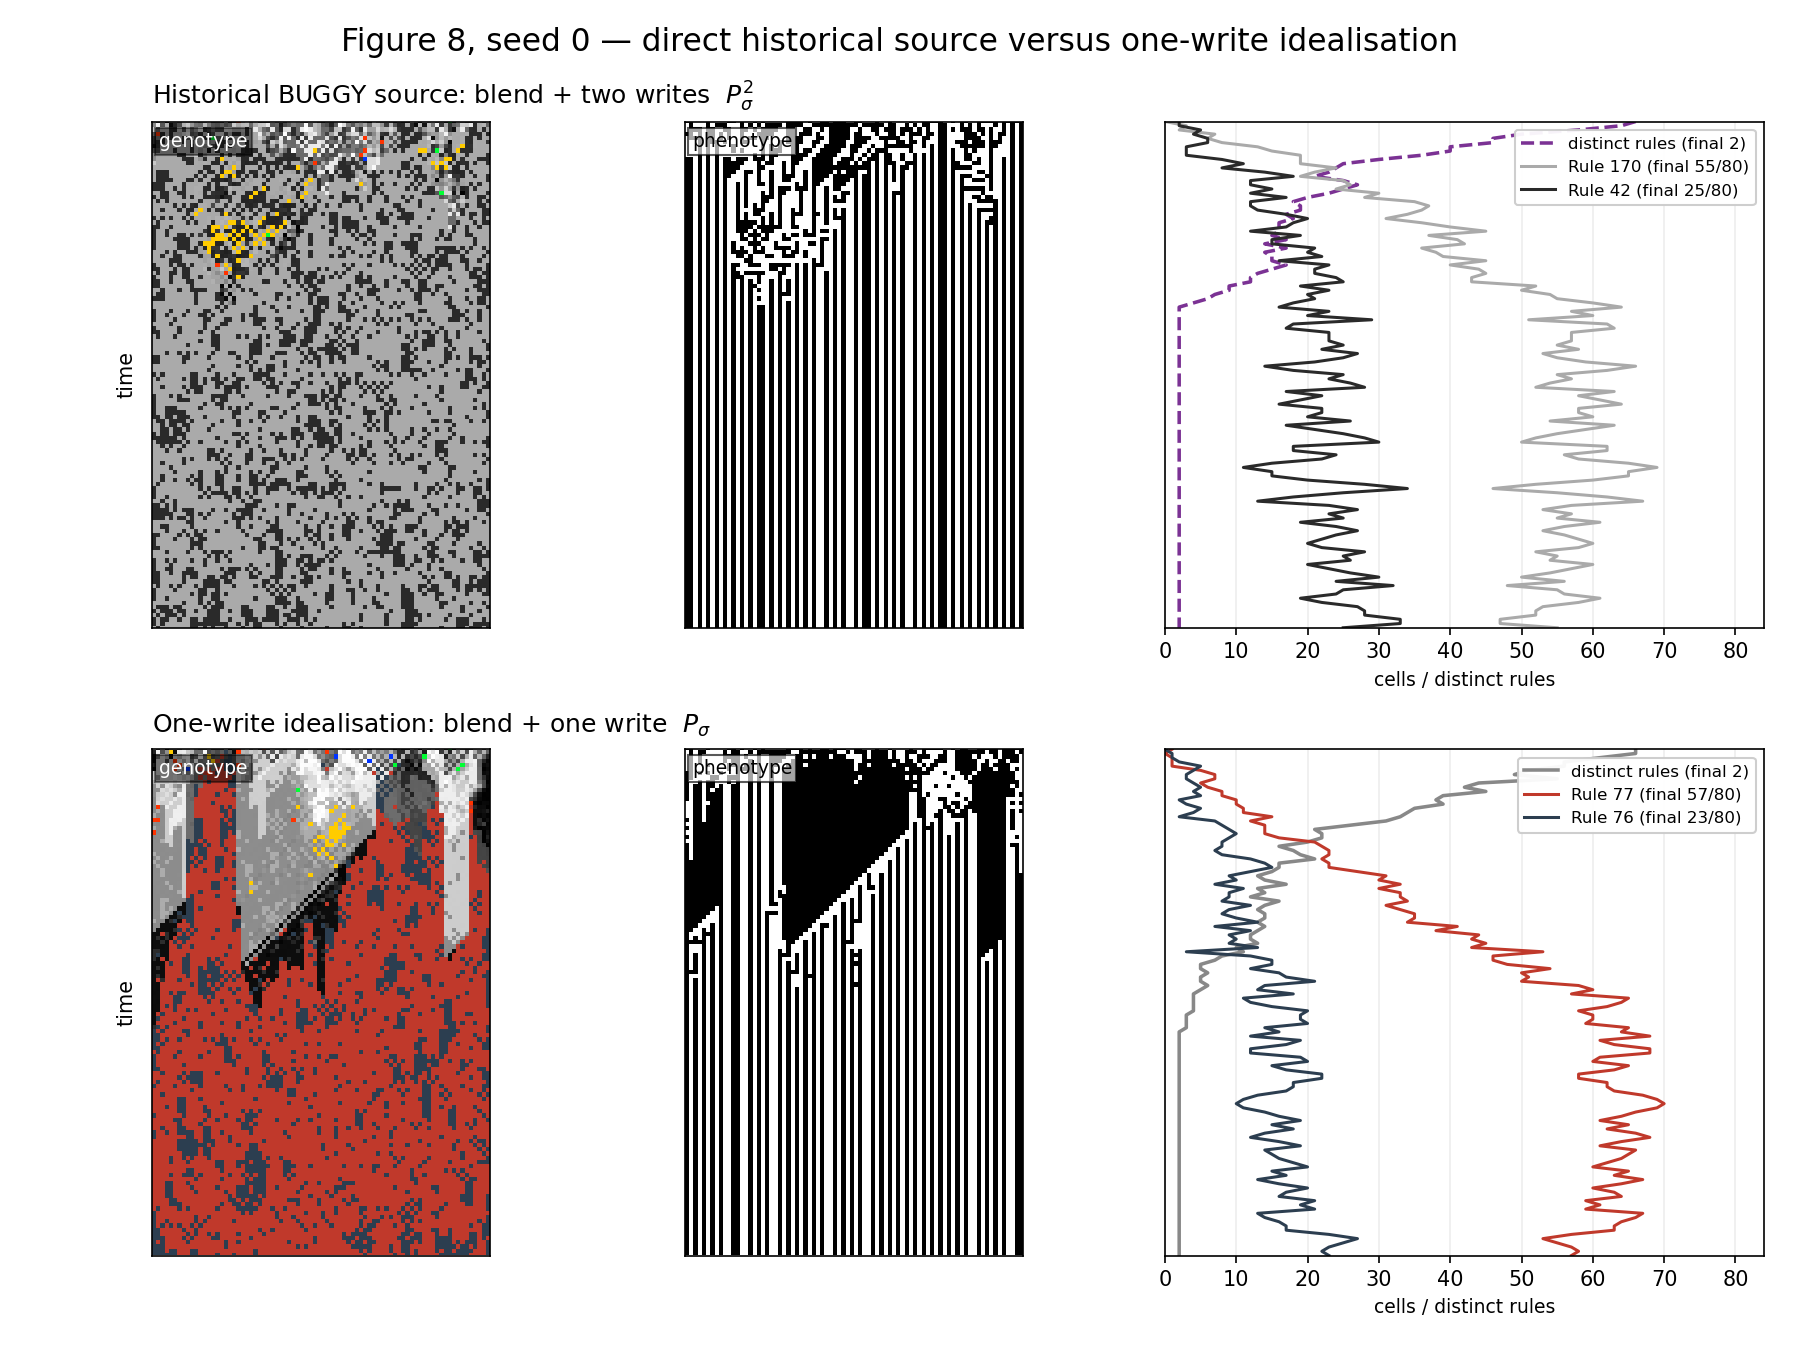
\includegraphics[width=\linewidth]{figures/fig8.png}
\caption{Figure~8 of the 2015 paper, reproduced---the family's accidental
first sighting, from the original erroneous mutation (one bit frozen). A
triptych on a shared time axis: genotype (left, coloured as in
Figures~\ref{fig:regimes}--\ref{fig:river}, well-known ECAs visible early),
phenotype (centre), and the population dynamics (right): the count of
\emph{distinct} rules (grey) collapses from tens to two, while the two
survivors---rules $170$ (red) and $42$ (dark)---rise and fluctuate as they
partition the field between them. The alternating population is what the
frozen bit preserves; this is the $k=1$ case of the $2^k$ count.}
\label{fig:figure8}
\end{figure}

\section{The Census}
\label{sec:census}

\subsection{Parity predicts death across all 20{,}256 orbits}

Theorems~\ref{thm:parity}--\ref{thm:lambda} are statements about fixed
points; the census asks whether the parity dichotomy governs \emph{dynamics}.
Reducing the family by the mirror symmetry gives $20{,}256$ orbits; running
each and recording extinction, the all-even class dies roughly five times as
often as the rest, and the death rate is monotone in the number of cycles
$k$. The measured proportion of the all-even class reproduces the
combinatorial $27.34\%$ to two decimal places
(Figure~\ref{fig:parity})---an independent confirmation that the class the
theorem picks out is the class the dynamics single out.

\begin{figure}[t]
\centering
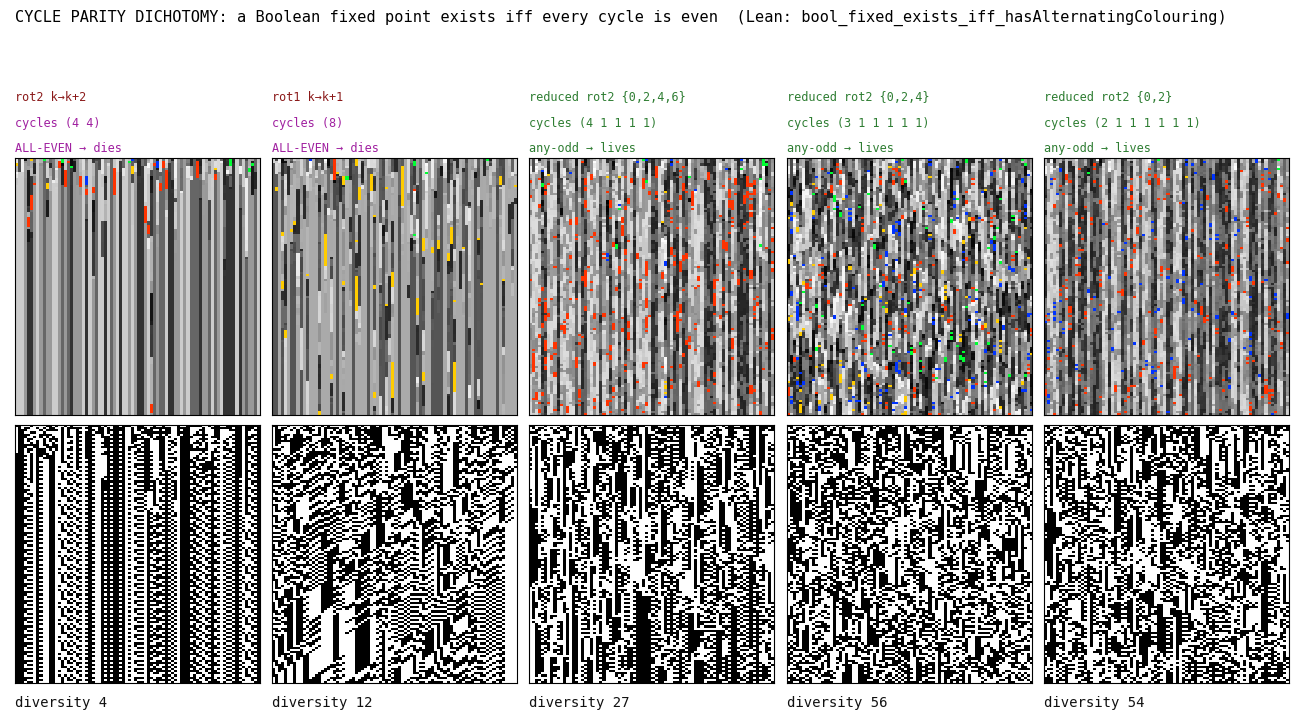
\includegraphics[width=\linewidth]{../../labs/M-aif-tokamak/compositions/parity-dichotomy.png}
\caption{The parity dichotomy, by example (the full census of $20{,}256$
orbits is summarised in the text). Five operators as genotype (top) and
phenotype (bottom) over time. \emph{Left:} the all-even operators
rotate$+2$ and rotate$+1$ possess fixed points (Theorem~\ref{thm:parity})
and, left to settle, are \emph{absorbed} onto them---rotate$+2$ collapses to
four rules, its $2^k = 2^2$ count. \emph{Right:} the any-odd operators
(reduced rotate$+2$, acting on a subset so the remaining positions are odd
one-cycles) possess no fixed point, cannot settle, and stay diverse. This
absorption is the operator left to itself; a neighbour-blend interrupter
reverses it for the $\gcd 2$ case (Figure~\ref{fig:lambda},
\S\ref{sec:interrupter}), and that reversal is the dynamical point.}
\label{fig:parity}
\end{figure}

\subsection{A prospective test: reduced rotate$+2$}

To guard against reading structure into a completed enumeration, we
registered a prediction before running it: the reduced $\text{rotate}{+}2$
operator, all of whose cycles are even, should fall on the possesses-fixed-
points, dies-preferentially side of the dichotomy. It does.

\section{The Operator Is a Bias, Not an Absorber}
\label{sec:interrupter}

\begin{figure}[p]
\centering
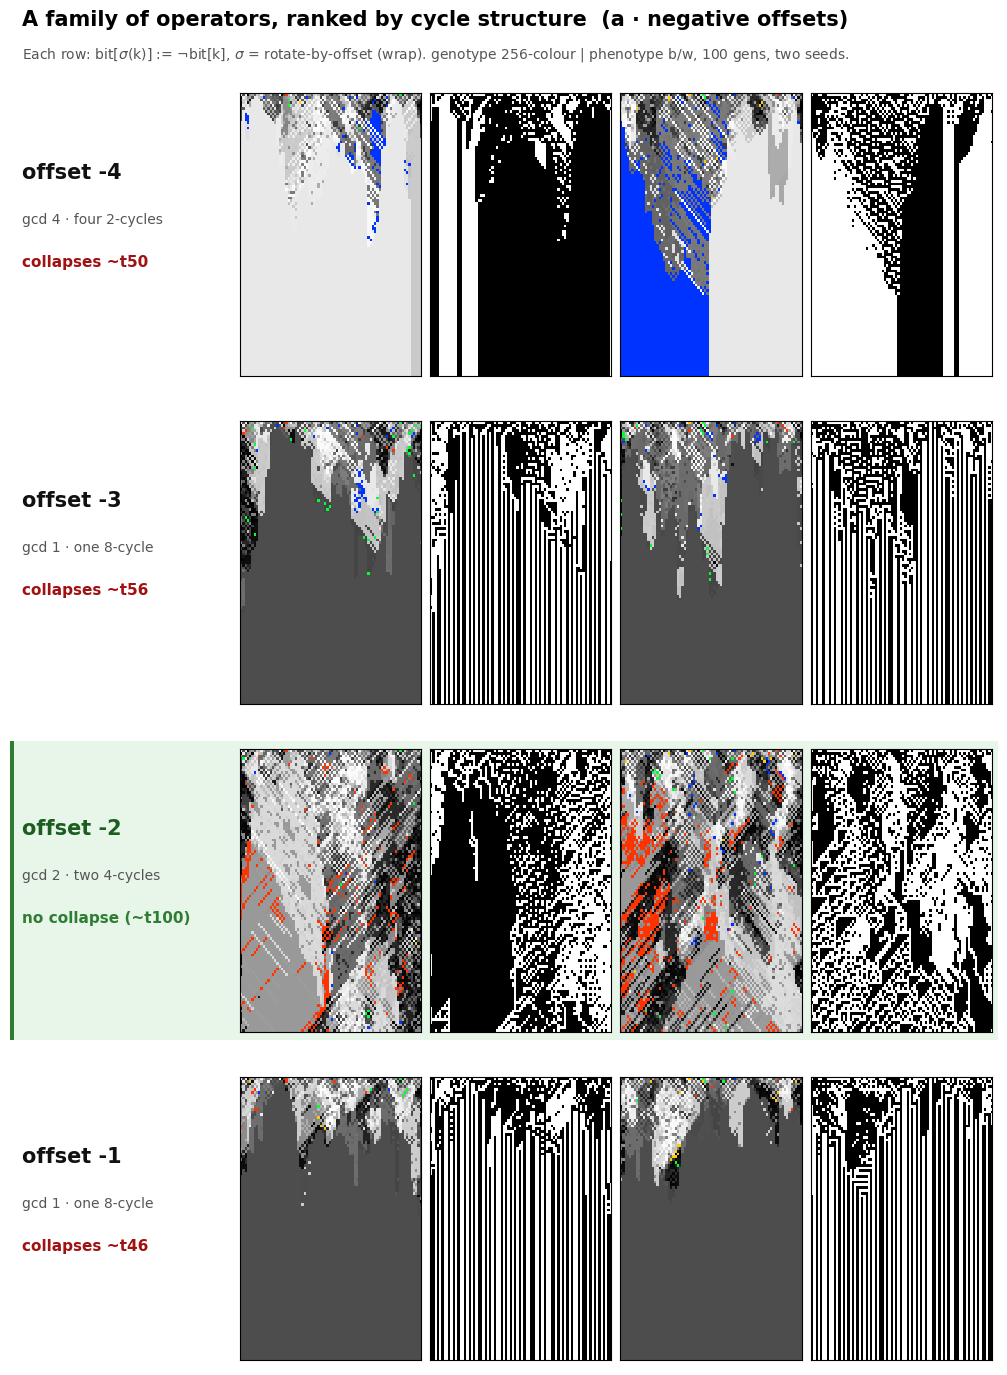
\includegraphics[height=0.92\textheight]{figures/survey_a.png}
\caption{\textbf{(a)~Negative offsets.} The rotation subfamily, ordered by
offset. Each row is one operator $\bit{\sig(k)} := \lnot\,\bit{k}$ with
$\sig$ a wrap rotation, shown for two seeds as genotype (256-colour) and
phenotype (black and white) over the first hundred generations. Every
non-trivial rotation is all-even and so possesses fixed points
(Theorem~\ref{thm:parity}); yet only $\gcd(\text{offset},8)=2$---offset
$\pm 2$, two $4$-cycles, highlighted green---sustains a rich edge-of-chaos
phase. The remaining rotations collapse to near-uniform fields within a few
dozen generations. Continued in panel~(b).}
\label{fig:eoc}
\end{figure}

\begin{figure}[p]
\ContinuedFloat
\centering
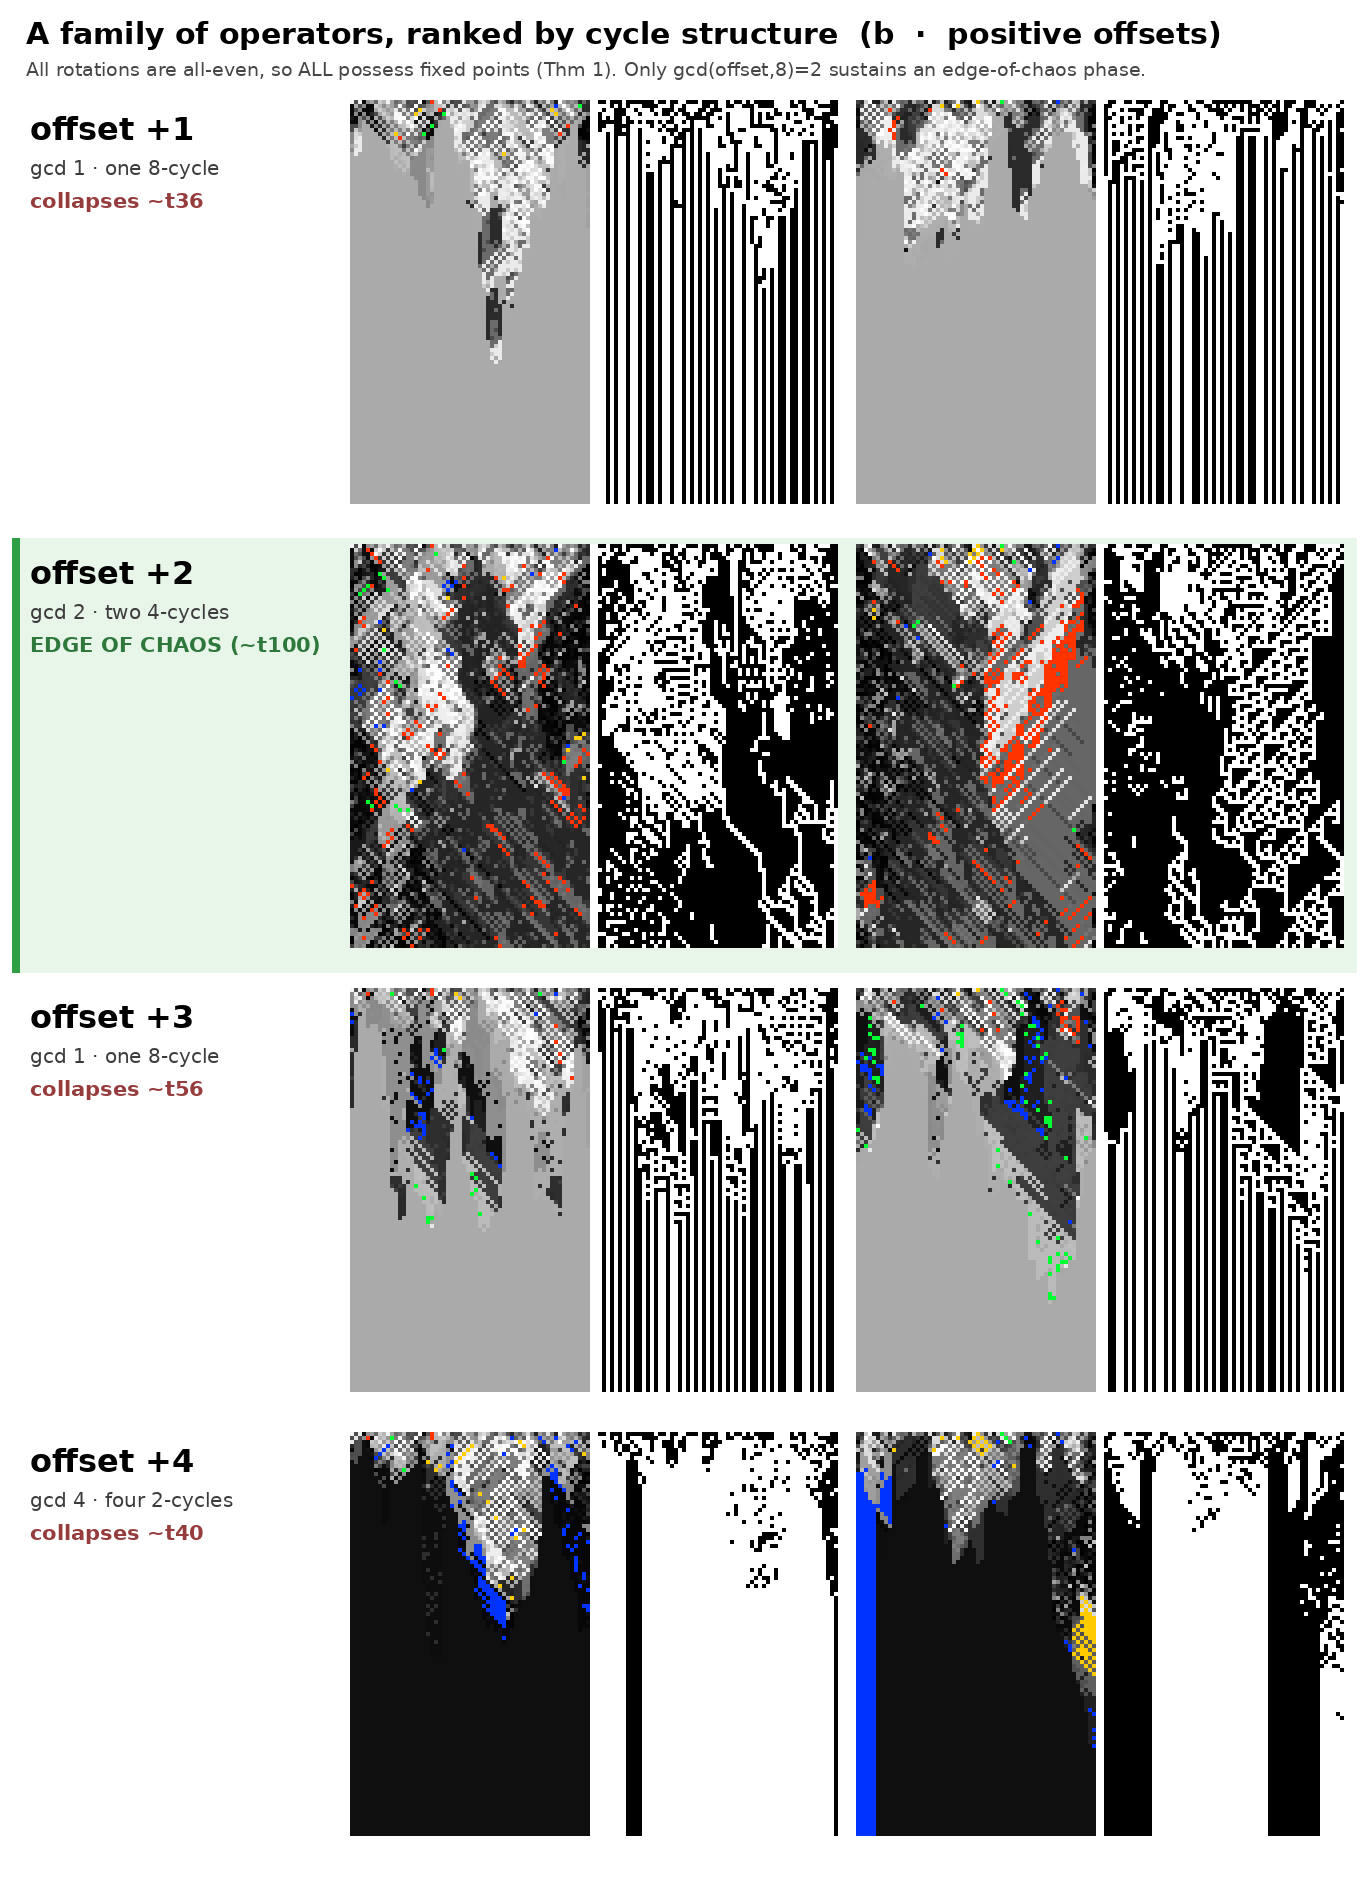
\includegraphics[height=0.92\textheight]{figures/survey_b.png}
\caption{\textbf{(b)~Positive offsets.} Continued from panel~(a). The pattern
is symmetric: offset $+2$ ($\gcd 2$, two $4$-cycles) sustains the
edge-of-chaos phase, the rest collapse. Possessing an attractor and living
near it are different properties, and this pair of pages is the whole paper
in one figure.}
\end{figure}

Possessing a fixed point (Theorem~\ref{thm:parity}) is not the same as
reaching one. Applied deterministically from a random initial rule, the
operator does not converge to its fixed point; because~\eqref{eq:prop} is a
bijection on bytes, a generic byte lies on a periodic orbit and simply
cycles. The operator therefore acts as a \emph{bias} toward $\lambda = 1/2$,
not an absorber onto it: it lowers the variance of activity and pulls toward
the critical value from either side, but it does not by itself hold a field
there.

The rotation family makes this concrete. Every non-trivial wrap rotation is
all-even and so possesses fixed points (Theorem~\ref{thm:parity}), yet only
offset $\pm 2$---$\gcd(2,8)=2$, two $4$-cycles---sustains a rich
edge-of-chaos phase (Figure~\ref{fig:eoc}), surviving to roughly a hundred
generations at high rule-diversity; the remaining rotations ($\gcd 1$ and
$\gcd 4$) collapse to near-uniform fields within a few dozen. Possessing an
attractor and living near it are different properties, and only the second
is visible in a drawing.

This last distinction can be \emph{measured}, with the population curve of
\S\ref{sec:lambda} as the instrument. Every rotation begins at peak
diversity---some seventy distinct rules in a random field---but the
$\lambda$-analogue then diverges sharply by cycle structure
(Figure~\ref{fig:lambda}): offset $\pm 2$ hold $\approx 31$ distinct rules
indefinitely, while every $\gcd 1$ and $\gcd 4$ rotation collapses to one or
two within sixty generations. The sustained edge-of-chaos of the $\gcd 2$
operators and the brief edge-of-chaos transient of the rest---read off the
drawings of Figure~\ref{fig:eoc} by eye---are thus separated by a factor of
fifteen in a single scalar. The curve that Figure~8 introduced, applied
across the family, is the order parameter.

\begin{figure}[t]
\centering
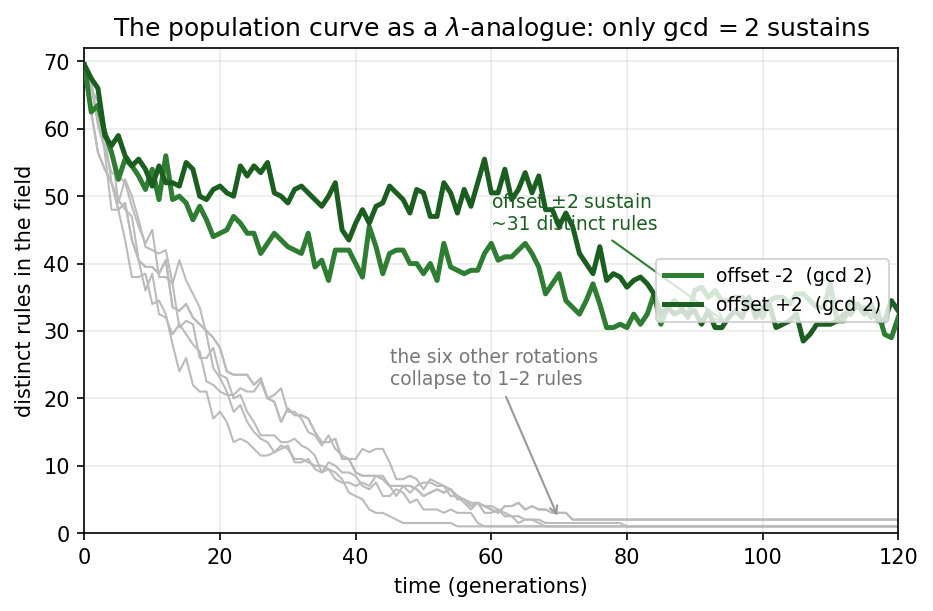
\includegraphics[width=\linewidth]{figures/lambda_analogue.png}
\caption{The population curve as an order parameter. Distinct rules in the
field over time, for the eight wrap rotations (two seeds each). All begin at
$\approx 70$; only the two $\gcd 2$ operators, offset $\pm 2$ (green),
sustain a large diverse population, while the six others collapse to one or
two rules. This is the sustained-versus-transient edge-of-chaos distinction
of Figure~\ref{fig:eoc}, made quantitative through the $\lambda$-analogue of
\S\ref{sec:lambda}. The interrupter is essential: left to settle without it,
these same all-even operators are absorbed onto their $2^k$ fixed points
instead (rotate$+2$ onto four; Figure~\ref{fig:parity}).}
\label{fig:lambda}
\end{figure}

Sustained structure requires an \emph{interrupter} --- a step that
occasionally declines to propagate. Composed with such a step (a
neighbour-blend that copies where neighbours agree, or a hold-when-active
gate), the operator's bias becomes a living regime: a diverse population of
rules held near $\lambda = 1/2$ rather than a single frozen byte or a
runaway orbit. The interrupter is what converts the fixed-point \emph{bias}
of the algebra into a sustained dynamical object. This resolves the apparent
tension between the census and the $\lambda$-analogue: they show the same
operator in its two regimes. In the census (Figure~\ref{fig:parity}), left
to settle, rotate$+2$ is \emph{absorbed} onto its four fixed points; with
the interrupter (Figure~\ref{fig:lambda}) it is held off them and sustains
tens of rules. Bias and absorption are two regimes of one operator, and the
interrupter selects between them.

Propagators do not compose usefully with one another, and this negative
result shapes what composition can do here. Each operator of
Equation~\eqref{eq:prop} negates every bit---$P_\sig(g)[j] = \lnot\,
g[\sig^{-1}(j)]$, a permutation of the eight coordinates followed by a global
flip---so under composition the flips cancel in pairs. The product
$P_\sig \circ P_\tau$ is a \emph{pure} coordinate permutation, with no
negation left in it: an absorber with $2^{c}$ fixed points for $c$ cycles
and none of the forced $\lambda = 1/2$ structure that made the single
operator interesting. An even number of propagators composes to such a bare
permutation, an odd number back to a single propagator $P_{\sig\tau\cdots}$;
either way the composite contains nothing the individual operators did not.
The family is flat under its own composition. We searched composites of two
and three operators for emergent structure and found none---the negation
that gives one operator its edge-of-chaos fixed point is exactly what a
second operator cancels---so the compositions that \emph{do} yield something
new must pair a propagator with a step of a different kind.

One such composition is worth exhibiting. Taking the offset-$+2$
propagator---the $\gcd 2$ operator of Figure~\ref{fig:eoc}---and composing
it with a construction step that reads the phenotype, matches it against
local templates, and falls back to the all-zero rule produces a
\emph{river}: a coherent band of alternating phenotype that drifts through a
disordered background and reappears in every seed (Figure~\ref{fig:river}).
Where the bare rotation collapses or orbits, this composition holds an
off-critical structure indefinitely---its trajectory varying with the seed,
its existence not. We report these two mechanisms here; a fuller catalogue
of composed operators is future work.

\begin{figure}[t]
\centering
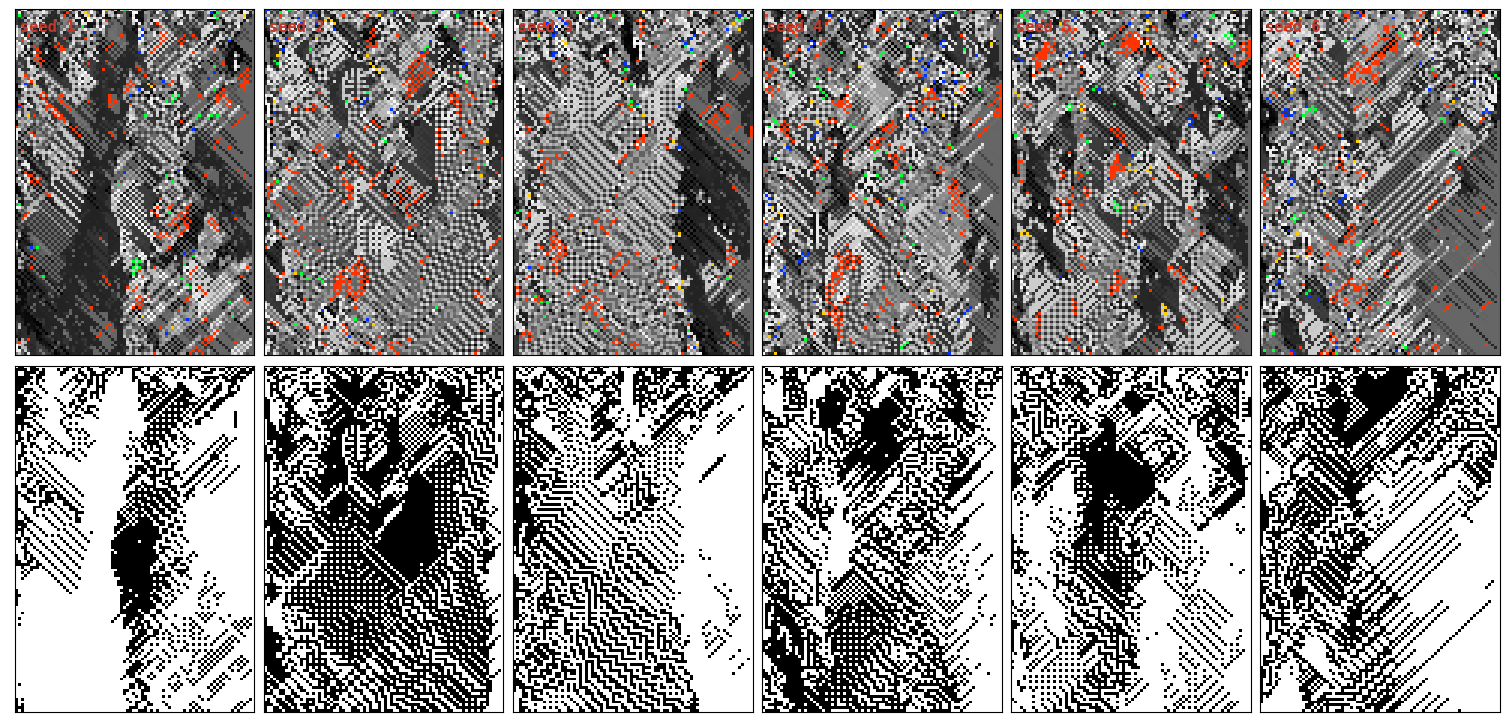
\includegraphics[width=\linewidth]{figures/river.png}
\caption{A \emph{river}: a composed operator sustains a reproducible
structure. The offset-$+2$ propagator, composed with a phenotype-reading,
template-matching construction (fallback: the all-zero rule), produces in
every seed a coherent band of alternating phenotype (bottom row) drifting
through a disordered background (genotype top, six seeds; genotype coloured
by rule as in Figures~\ref{fig:regimes}--\ref{fig:eoc}---greyscale by byte
value, with well-known ECAs highlighted, red~$=$~Rule~110). The band's
trajectory varies with the seed; its presence does not.
Where the bare rotations collapse or orbit (Figure~\ref{fig:eoc}), this
composition holds an off-critical structure indefinitely.}
\label{fig:river}
\end{figure}

\section{Why Distance Geometry Cannot See This}
\label{sec:metrics}

The classification is a conjugacy invariant of $\sig$ --- cycle type ---
and no distance on the state space or the rule space is a function of it.
This has a blunt consequence: the standard complexity and compression
measures cannot separate the classes. A unanimous cast (an all-even $\sig$
with $k=0$\,\ldots\ a single surviving byte, $2^0 = 1$) reads to a
population-diversity measure as maximally dead, though it is maximally
selected; a frozen periodic genotype scores a lower statistical complexity
$C_\mu$ \parencite{crutchfield1989inferring} than Rule~110; gzip codelength
rates a self-similar rule as noise. Each of these is a distance, and the
property is a parity. This is the whole of what an extended battery of
negative metric results amounts to, and it is an explanation rather than a
finding: the result is a theorem \emph{because} it is not a statistic.

\section{Limits}
\label{sec:limits}

The theorems are the Boolean case and are exact; the dynamical claims are
narrower. The census is a single reduction of one operator family
($S_8$, radius one, one value map); the bias-not-absorber behaviour and the
interrupter are reported at limited seed counts and invite a fuller
treatment. The substrate the object sits in is not itself new
(\S\ref{sec:object}), and $\lambda$ is one order parameter among several
\parencite{wuensche1999classifying}; we make no claim that it is
sufficient, only that here it is \emph{derived}. What is new, and what we
rest the paper on, is the object of Equation~\eqref{eq:prop} and the
fixed-point structure that places Langton's critical value at
$\lambda = 1/2$ as a matter of proof.

\section{Conclusion}
\label{sec:conclusion}

The characterisation promised in \S\ref{sec:object} has two halves. The
first is static and exact: which operators possess fixed points (the
all-even ones), how many ($2^k$), and where they lie (Langton's
$\lambda = 1/2$, always). The second is dynamic, and it is precisely what
the static half cannot supply---because every fixed point sits at
$\lambda = 1/2$, the classical parameter is silent on the difference between
an operator that sustains a diverse edge-of-chaos population and one that
collapses. The population curve, the $\lambda$-analogue of
\S\ref{sec:lambda}, is the order parameter that speaks: it separates
sustained from transient edge-of-chaos across the rotation family by a
factor of fifteen (Figure~\ref{fig:lambda}), and it revalues the search that
produced the family in the first place. The operator of
Figure~\ref{fig:regimes} that recovers Rule~110---the universal rule, the
naive prize of a search for computational intelligence---does so by
concentrating the field onto it ($38\%$ of cells), and pays for the
recovery in diversity: it sustains fewer distinct rules ($\approx 18$) than
its foil, which never finds Rule~110 at all yet holds a richer population
($\approx 23$). Recovering a universal rule and sustaining an open-ended
search are, in this family, opposed---and the measure that completes the
static classification is the same one that tells them apart.

\printbibliography
\end{document}
